\documentclass[12pt]{article}%
% \documentclass[nofootinbib,preprint,floatfix,endfloats]{revtex4} % ,endfloats,floatfix
%\documentclass[12pt,a4paper,final]{iopart}

\usepackage[utf8]{inputenc}
\usepackage{nima,graphicx,amsmath,amssymb,color}%,hyperref}
\usepackage{mathrsfs}
%\usepackage{graphicx}
\usepackage{comment}
\usepackage{setspace}
\newcommand{\Ls}{\mathscr{L}}

\newcommand{\lrto}{\leftrightarrow}
 \marginparwidth 0pt
 \oddsidemargin  0pt
 \evensidemargin  0pt
 \marginparsep 0pt
 \topmargin   -0.25in 
\textwidth   6.5in
 \textheight  9.0in
\newcommand{\RNum}[1]{\uppercase\expandafter{\romannumeral #1\relax}}
\newcommand{\outNim}[1]{}
%

\begin{document}
\title{Simulation code}
\maketitle
\tableofcontents

\section{Transition Point}
\subsection{Verifying the Scaling with $N$ and $L$}
To see if th predicted transition point behavior $\tilde{r}^c \propto N^{1/3}L^{-1/2}$ is accurate, we test it once on networks with a fixed number of nodes $N=50$ and on networks with approximately fixed $750<L<1250$. 
We verified that the curves of $d\log\be{l}/d\log r_L$ indeed collapse well when $r_L/r_N$ is scaled by $\tilde{r}^c$ (Fig. \ref{fig:trans-nl}). 

\begin{figure}
    \centering
    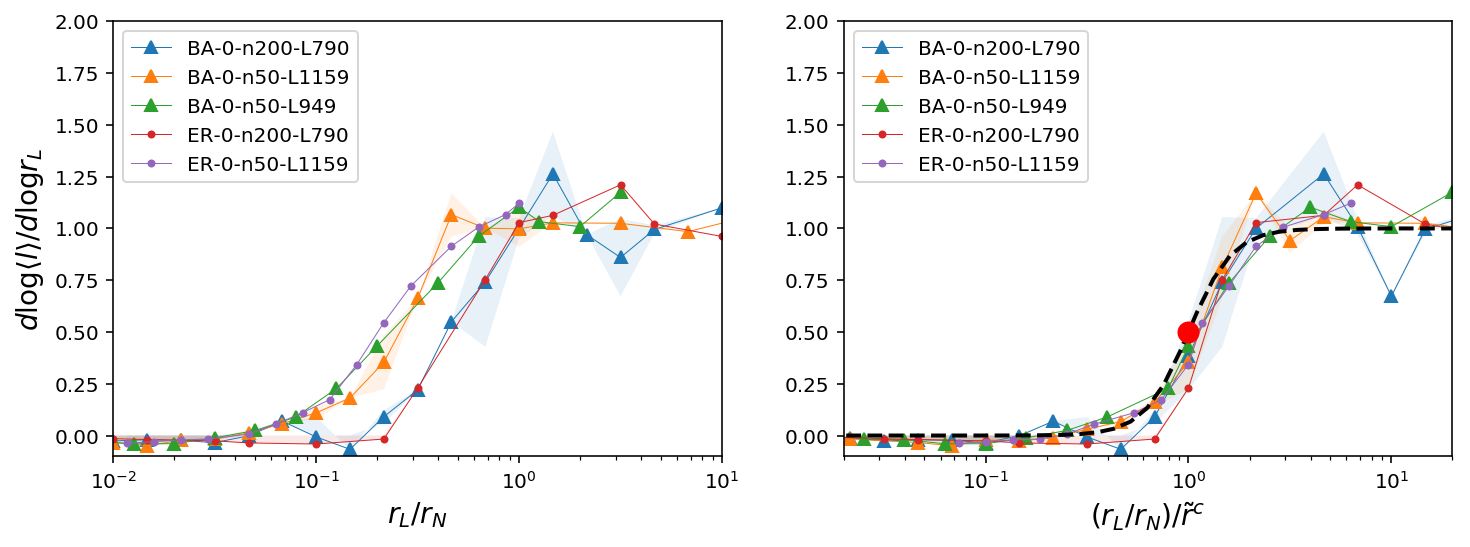
\includegraphics[width=.7\textwidth]{fig-09-19/phase-collapse-N.png}
    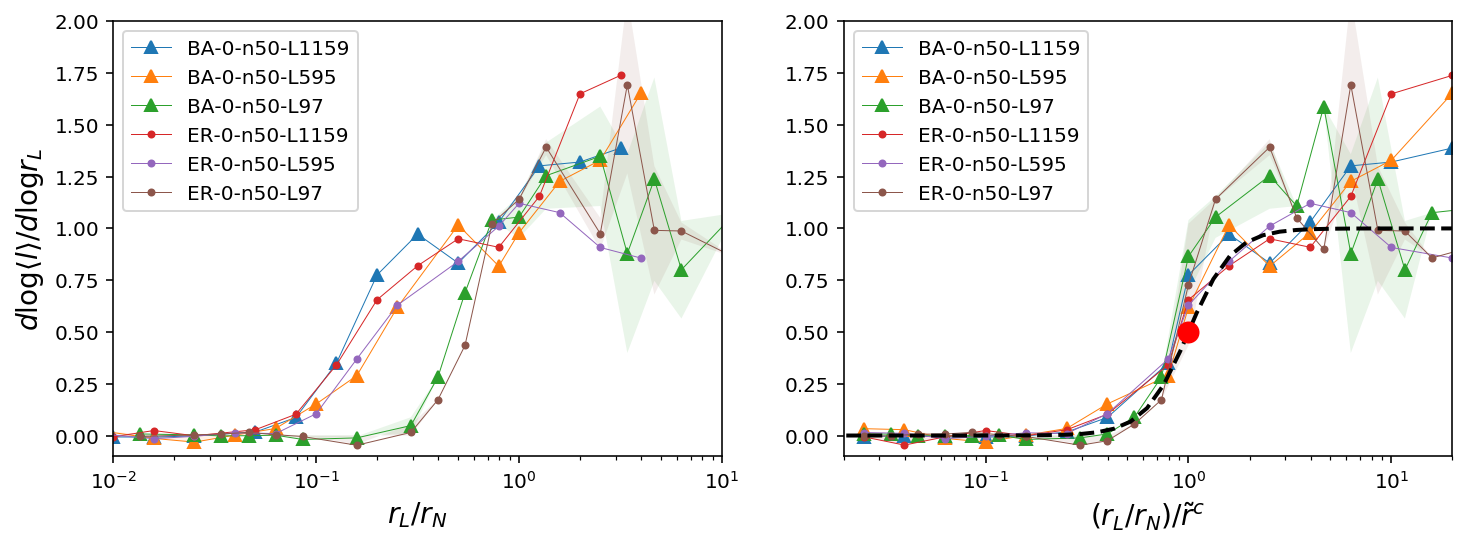
\includegraphics[width=.7\textwidth]{fig-09-19/phase-collapse-L.png}
    \caption{\scriptsize 
    Behavior of the transition point for varying $N$ (top) and $L$ (bottom) separately. 
    The plots on the left and right column are before and after scaling by $\tilde{r}^c$, respectively.
    The rescaling results in a good collapse of the curves. 
    No discernible difference is observed between scale-free (BA) and random (ER) networks. 
    }
    \label{fig:trans-nl}
\end{figure}
No measurable difference based on degree distribution was observed in the simulations when comparing random and scale-free networks (Fig. \ref{fig:trans-nl}).


\subsection{Parameters}
The model in Eq. (1) is a smooth approximation of a system with hard-wall potentials for the repulsive forces. 
As such, the transition point exhibits some dependence on the parameters of the potential, such as the ratio of the spring constant to the repulsion amplitude, $k/A_{L,N}$ in links and nodes. 
This is because, with a smooth potential, the average distance between adjacent nodes or links depends on the magnitude of forces between them. 
For instance, in the weakly interacting regime, adjacent nodes will not be exactly $2r_N$ apart from each other, and the exact distance depends on the $k/A_N$ ratio. 
For the node-node repulsion between two adjacent nodes $i$ and $j$ with distance $r_{ij}$ from each other we have 
\begin{align}
    |F_{NN}| = A_N\pr{{r_{ij}\over 2r_N}}^{p-1} \exp[\left[-\pr{{r_{ij}\over 2r_N}}^{p} \right]
\end{align}
In a regular lattice, this force is offset by the elastic force $2r_{ij} k$ in the links in the weakly interacting phase.
Thus, the equilibrium distance between adjacent nodes is found by solving ($y\equiv r_{ij}/(2r_N)$
\begin{align}
{4r_N k \over A_N} &= y^{2-p} e^{-y^p}    
\end{align}
For example, if we choose $p=2$, $k/A_N = 0.1 $ and $r_N=1$ the equilibrium distance satisfies 
\[{r_{ij}\over 2 r_N} = \sqrt{- \log {4r_N k\over A_N}} \approx 0.96\]
This would affect the location of the transition point.
Unlike the node distance, which is directly affected by the elastic forces in the links, the average link distance is only affected deep in the strongly interacting phase. 
Thus, the choice of $k/A_N$ should be such that it results in $r_{ij} \approx 2r_N$. 

\outNim{
However, we have the same kind of potential for link repulsion and as long as the choice of $k/A_{L,N}$ and $p$ are the same for links and nodes, we expect the ratio of $r_{ij}/(2r_N)$ for adjacent nodes to be similar to $r_{lm}/(2r_L)$ for adjacent links, allowing us to ignore the effect of  
The transition point has some  dependence on the choice of parameters. 
$k/A_L$ ratio, as well as $A_L/A_N$. 
I am still unable to reproduce exactly the transitions I had observed in the 040518 data, which seems to be a copy of the 032818 and 032918 data. 
Now I am able to, but the dependence on $k/A$ is still enigmatic. 
} 

% But there does seem to be a strong dependence on the the ratio of the link spring constant $k$ to the link repulsion amplitude $A_L$.

The shift in the transition point for when varying $k/A_N$ stem from the average distance between adjacent nodes being a function of $k/A_L$ ratio.
Indeed, examining the lattice in the weak phase reveals that the average size of the network changes with the $k/A_L$ ratio. 
Scaling the $r_L/r_N$ ratio by how much the size of the layout has changed results in an almost perfect collapse of the order parameter for the lattice. 
To be precise, the ``effective'' scaling of the network size can be found by measuring the ratio of the average link length to twice the link thickness 
\[{r_L^{eff}\over r_L} = {\be{l(r_L)}\over 2 r_L}\]
where $r_L$ is deep in the strong phase. 
\begin{figure}
    \centering
    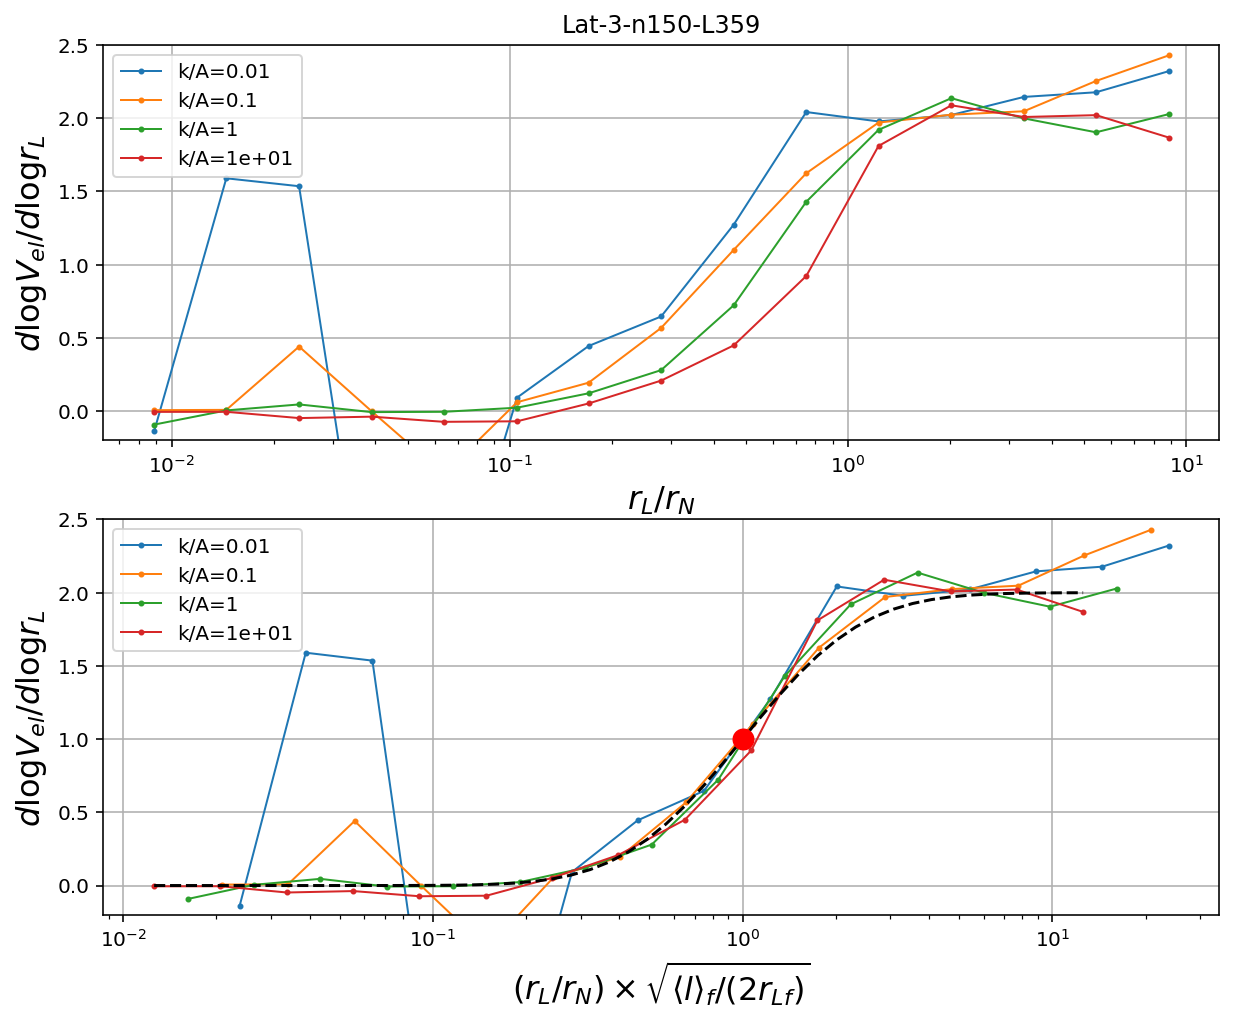
\includegraphics[width=.7\textwidth]{fig-09-19/Lat-kA-scaled-fit.png}
    \caption{\scriptsize {\bf Collapsing the $k/A_L$ curves for lattice:} the order parameter $d\log \be{V_{el}} /d \log r_L $ shows different transition points for the same lattice with different values of $k/A_L$.
    However, changing $k/A_L$ also changes the layout size, which indicates that instead of $r_L$ the layouts have an ``effective'' $r_L^{eff}(k/A_L)$.  
    This $r_L^{eff}$ scales with $\be{l}^{1/2}$ and rescaling $r_L$ by this growth ratio collapses the transition curves onto a standard error function.}
    \label{fig:l-kA-lat}
\end{figure}


% \outNim{
\begin{figure}
    \centering
    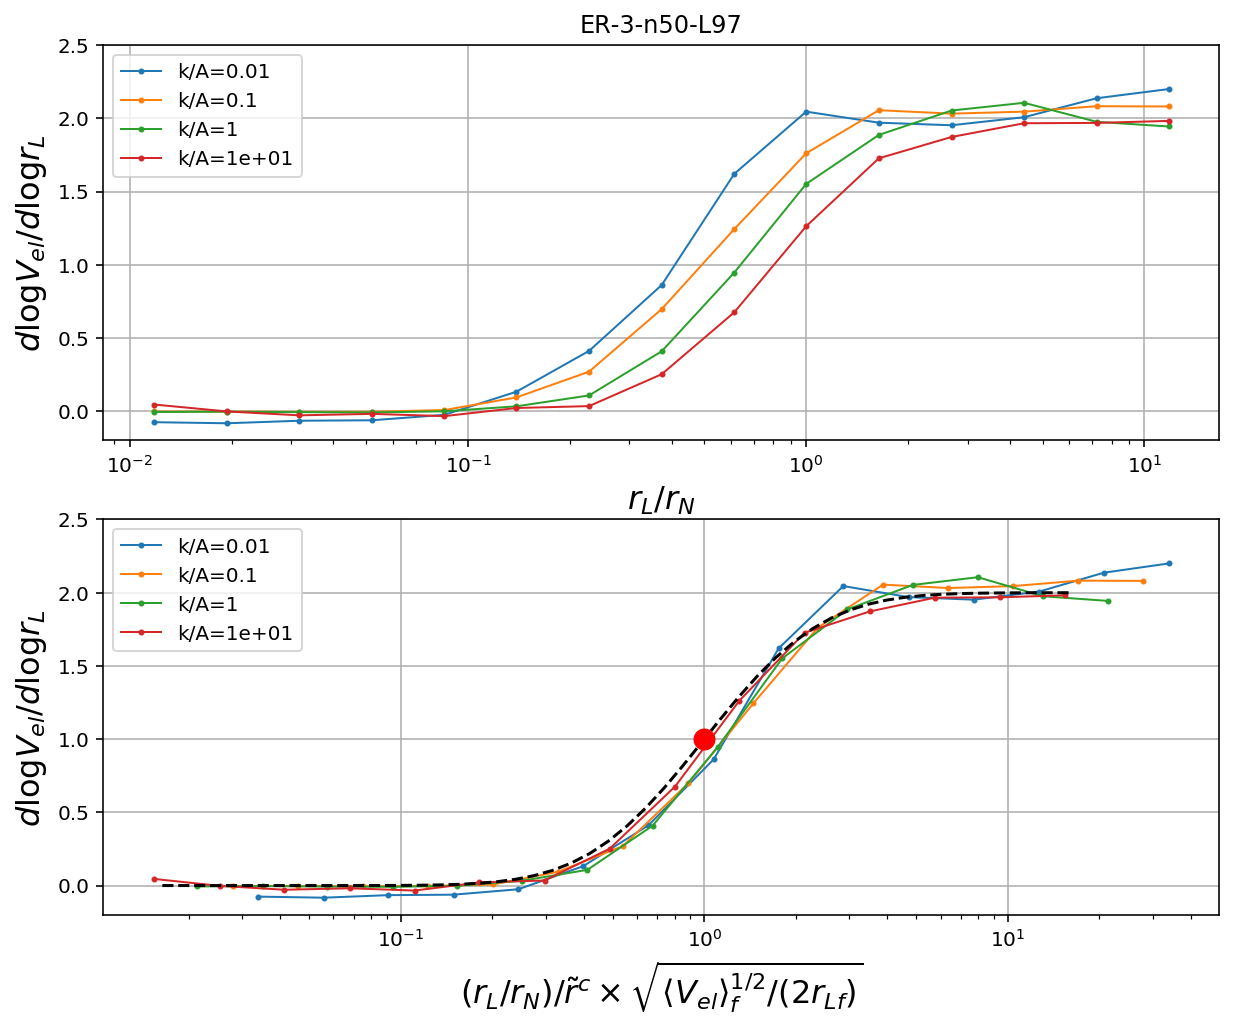
\includegraphics[width=.7\textwidth]{fig-09-19/ER-kA-scaled-fit.png}
    \caption{\scriptsize {\bf Collapsing the $k/A_L$ curves for ER:} the order parameter $d\log \be{V_{el}} /d \log r_L $ for different values of $k/A_L$ collapses slightly differently from the lattice. 
    The effective $r_L^{eff}$ scales with the elastic potential $\be{V_{el}}^{1/4}$ and rescaling $r_L$ by this growth ratio and $\tilde{r}^c$ collapses the transition curves onto a standard error function.}
    \label{fig:l-kA-er}
\end{figure}
% }%%%%%

\subsubsection{Effect of power in the repulsive potential}
There doesn't seem to be much dependence on the steepness through the power $p$ in the $V_{NN} = \sum_{n,m} A_N \exp[|\Delta x_{mn}/2 r_N|^p $ (Fig. \ref{fig:POWn}).


\begin{figure}
    \centering
    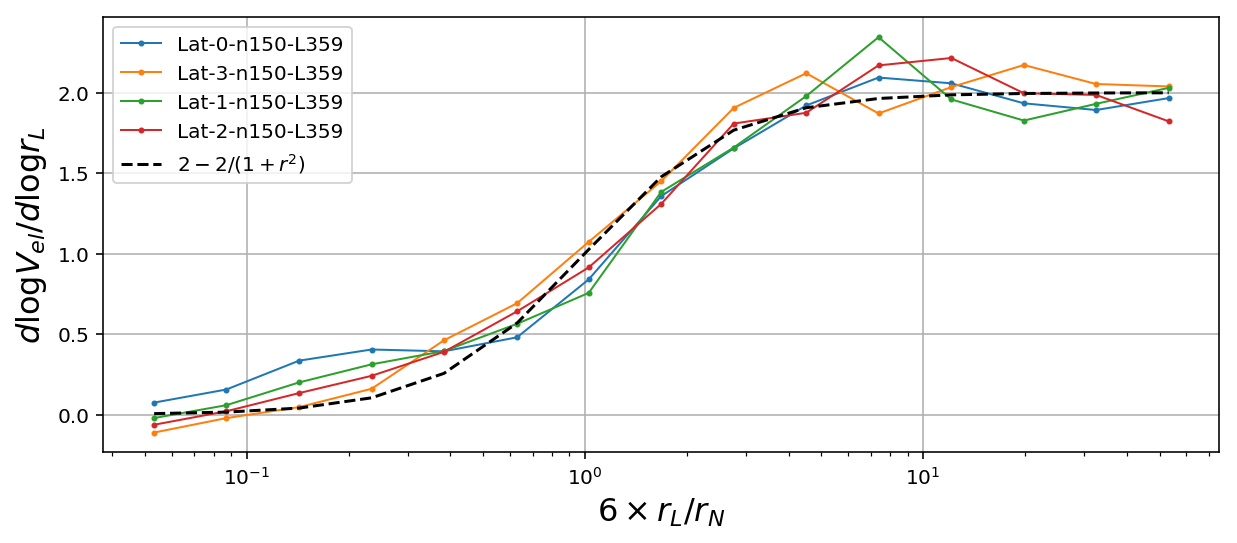
\includegraphics[width=.7\textwidth]{fig-09-19/Lat-POWn.png}
    \caption{\scriptsize {\bf The effect of node potential steepness:} Simulation of the same lattice with different powers $p$ in the $V_{NN} = \sum_{n,m} A_N \exp\left[|\Delta x_{mn}/2 r_N|^p \right]$. 
    The values of $p$ were $2,3,4,6$ for Lat-0,Lat-1,Lat-2,Lat-3, respectively.
    As we see, there is no significant effect on the transition point arising from $p$.}
    \label{fig:POWn}
\end{figure}
\outNim{
\begin{figure}
    \centering
    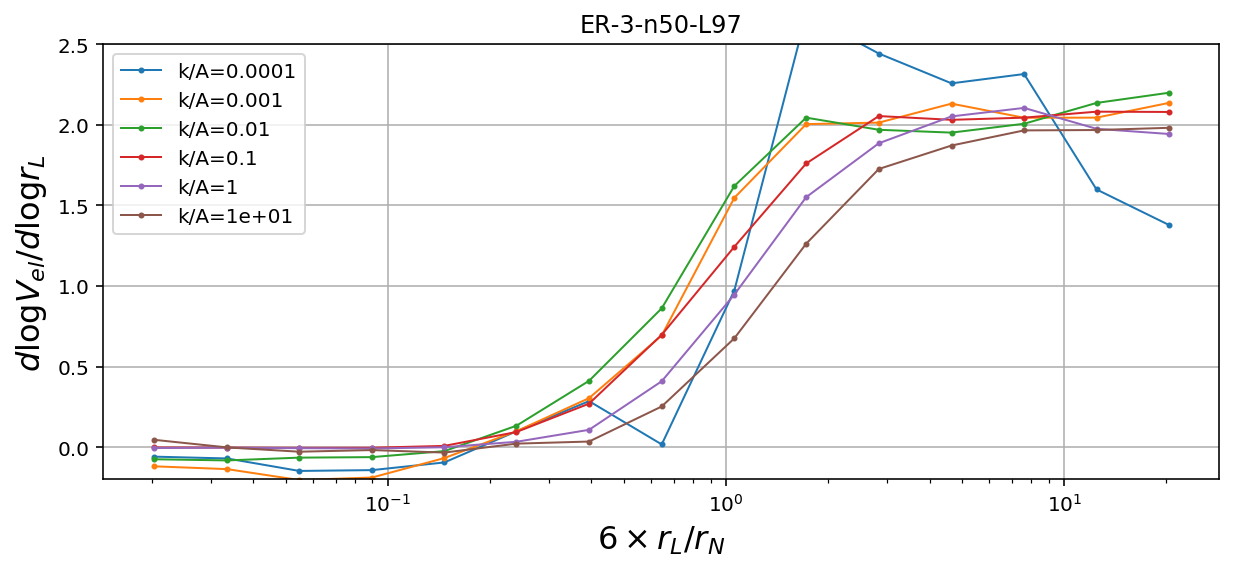
\includegraphics[width=.7\textwidth]{fig-09-19/ER-kA.png}
    \caption{\scriptsize {\bf The effect of ratio of link spring constant to link repulsion amplitude:} Simulation of the same ER network with different values of $k/A_L$.
    %The transition point seems to move by a factor proportional to $log(k/A)$.
    }
    \label{fig:kA}
\end{figure}
}%%%%%%

\subsubsection{Number of Link Segments}
The numerical simulations are done by discretizing the links into a number of interlaced, interacting beads. 
This approximation will introduce finite-size effects and the measured transition point does have some dependence on the number of link segments (Fig. \ref{fig:er-segs}). 

\begin{figure}
    \centering
    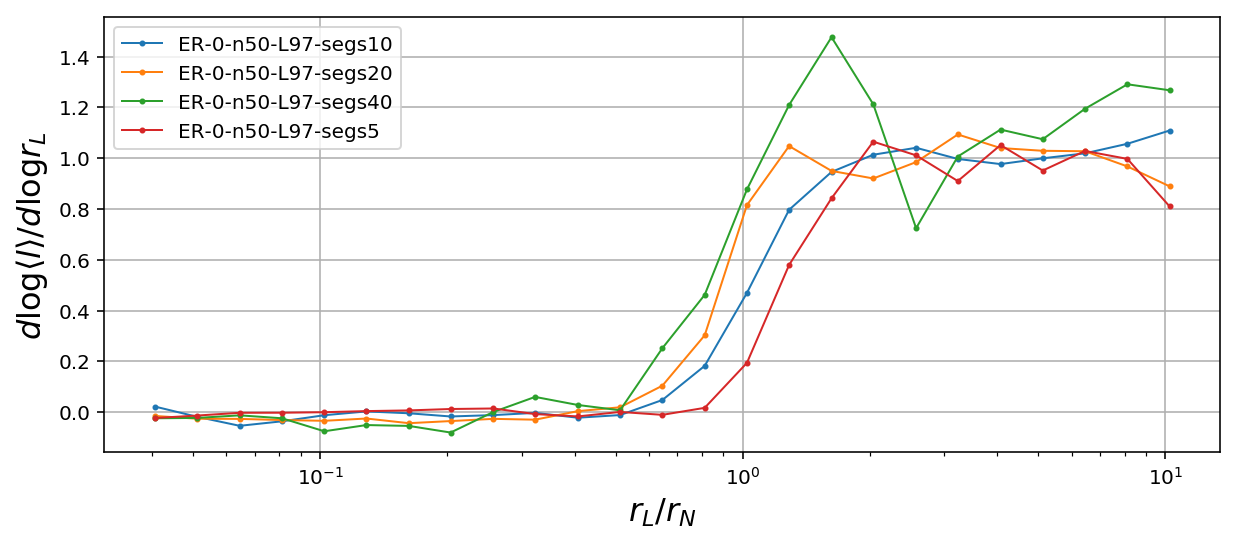
\includegraphics[width=.7\textwidth]{fig-09-19/ER-segs.png}
    \caption{\scriptsize The effect of number of discrete link segments used in simulations.
    Increasing the number of segments slightly reduces the with of the transition region, and makes the transition slightly sharper. 
    }
    \label{fig:er-segs}
\end{figure}

\section{Curvature\label{ap:curvature}}
The curvature of a curve $\gamma(s)$ measures how much the tangent of the curve $T(s) \equiv \gamma'(s)$ changes along the path. 
Here $s$ is an affine parameter, like the arc-length.  
Hence, the extrinsic curvature $\kappa(s)$ is given by magnitude of the second derivative of the curve 
\begin{equation}
    \kappa(s) = |T'(s)| = |\gamma''(s)|
\end{equation}
The path is defined as $\gamma(s) = (x(s),y(s),z(s))$ in Cartesian coordinates and the tangent related to the gradient of $\gamma(s)$
\begin{align}
    T(s) &= {d \gamma(s) \over ds} = \vec{x}'(s)\cdot \vec{\del} \gamma(s) = x'(s)\hat{x}+y'(s)\hat{y}+z'(s)\hat{z} 
\end{align}
Since $s$ is the affine parameter and $ds^2 = dx^2 + dy^2 + dz^2$, we always have $|T(s)|=1$. 
For arbitrary parametrization, we have $T = \gamma'/|\gamma'|$.
Therefore, just as in circular motion, $T'(s)$ will be perpendicular to $T(s)$ and related to the radius of curvature. 
Taking the second derivative, the curvature can be summarized as 
\begin{equation}
    \kappa = {|\gamma'\times \gamma''|\over |\gamma'|^{3}}
\end{equation}
In practice, for measuring link curvature, we can implement this by measuring the cross product of the tangent vector $\gamma'(s)$, calculated for every link segment, and the second derivative $\gamma''(s)$ and dividing by $|\gamma'(s)|^3$. 
Note that $\kappa(s) = 1/R(s)$ with $R(s)$ being the radius of curvature. 
But, taking the same curve and scaling it up will increase the radius of curvature and decrease the curvature. 
Therefore, to compare curvature in networks of various sizes we rescale the curvature by the average link length $\be{l}$ and measure $\be{l}\kappa(s) = \be{l}/R(s)$.
\end{document}